\documentclass[12pt,a4paper]{article}
\usepackage[UTF8]{ctex}
\usepackage{amsmath,amssymb}
\usepackage{xcolor}
\usepackage{hyperref}
\usepackage{geometry}
\usepackage{graphicx}
\geometry{margin=2.5cm}

\title{Classical While / 经典循环}
\author{QuoNic}
\date{}

\begin{document}
\maketitle

\begin{center}
\textbf{Language / 语言特性} | 难度：初级 | 预计时间：5 分钟
\end{center}

\tableofcontents
\newpage

\section{为什么需要？}

经典循环是在量子程序中使用经典 while 循环。

\subsection{经典局限}
\begin{itemize}
  \item 经典循环无法直接用于量子态
  \item 需要先测量量子态
\end{itemize}

\subsection{量子优势}
\begin{itemize}
  \item 经典循环可以在量子程序中使用经典迭代
  \item 是混合编程模型的基础
  \item 支持量子-经典混合算法
\end{itemize}

\subsection{实际应用}
\begin{itemize}
  \item 量子-经典混合算法
  \item 变分量子算法
  \item 量子优化
\end{itemize}

\section{快速上手}

\begin{verbatim}
from quonic import qgate, cshow
from quonic.gates import H

# 经典循环
while True:
    qgate(H, 0)
    result = cshow()
    if result == '1':
        break
print('Got 1!')
\end{verbatim}

\textbf{预期输出}：
\begin{verbatim}
Got 1! (after 2 iterations on average)
\end{verbatim}

\section{原理详解}

\subsection{电路图}

\begin{center}
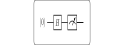
\includegraphics[width=0.6\textwidth]{../../images/cwhile_circuit.svg}
\end{center}

\subsection{数学推导}

经典循环：
\begin{equation}
\text{while } condition: \text{ do } A
\end{equation}

其中 $condition$ 是经典条件。

\subsection{几何解释}

经典循环在每次迭代中制备量子态、测量、检查条件。直到条件满足才停止。

\section{代码详解}

\begin{verbatim}
from quonic import qgate, cshow
from quonic.gates import H

# cshow() 返回经典测量结果
# while 循环直到条件满足
while True:
    qgate(H, 0)
    result = cshow()
    if result == '1':
        break
print('Got 1!')
\end{verbatim}

\section{进阶用法}

\subsection{场景 1：迭代优化}

\begin{verbatim}
from quonic import qgate, cshow
from quonic.gates import Ry

# 迭代优化
theta = 0.0
for i in range(100):
    qgate(Ry(theta), 0)
    result = cshow()
    if result == '1':
        theta -= 0.1
    else:
        theta += 0.1
\end{verbatim}

\subsection{场景 2：量子随机数生成}

\begin{verbatim}
from quonic import qgate, cshow
from quonic.gates import H

# 量子随机数生成
random_bits = []
for _ in range(8):
    qgate(H, 0)
    result = cshow()
    random_bits.append(result)
print(f'Random bits: {random_bits}')
\end{verbatim}

\section{适用场景}

\subsection{量子-经典混合算法}

经典循环用于量子-经典混合算法中的迭代优化。例如，VQE、QAOA 等变分算法需要迭代优化。

\subsection{量子随机数生成}

经典循环用于量子随机数生成。多次制备量子态、测量，收集随机比特。

\section{常见问题}

\subsection{经典循环和量子循环有什么区别？}

经典循环基于经典条件，量子循环基于量子测量结果。经典循环不会破坏量子态。

\subsection{经典循环会破坏量子态吗？}

不会。经典循环基于经典条件，不涉及量子测量。

\section{学习路径}

\subsection{前置知识}
\begin{itemize}
  \item 量子测量
  \item 经典编程
  \item 量子比特
\end{itemize}

\subsection{继续学习}
\begin{itemize}
  \item 量子条件分支（qif）
  \item 变分量子算法
  \item 量子-经典混合算法
\end{itemize}

\section{完整示例代码}

\subsection{示例 1：基本经典循环}

\begin{verbatim}
from quonic import qgate, cshow
from quonic.gates import H

while True:
    qgate(H, 0)
    result = cshow()
    if result == '1':
        break
print('Got 1!')
\end{verbatim}

\section{下载}

\begin{itemize}
  \item [cwhile.py](https://github.com/ChrisLee0721/QuoNic/blob/main/examples/cwhile/cwhile.py)
\end{itemize}

\end{document}
